\documentclass[a4paper,12pt]{article} 

%%% Работа с русским языком
\usepackage{cmap}                           % поиск в PDF
\usepackage{mathtext} 			 	       % русские буквы в формулах
\usepackage[T2A]{fontenc}               % кодировка
\usepackage[utf8]{inputenc}              % кодировка исходного текста
\usepackage[english,russian]{babel}  % локализация и переносы
\usepackage[left=2cm,right=2cm,
    top=2cm,bottom=3cm,bindingoffset=0cm]{geometry}
\usepackage{wrapfig}
\usepackage{gensymb}
\usepackage{textcomp}
\usepackage{multirow}
\usepackage{amsmath,amsfonts,amssymb,amsthm,mathtools} % AMS
\usepackage{euscript}	 % Шрифт Евклид
\usepackage{mathrsfs} % Красивый матшрифт
\usepackage{graphicx}%Вставка картинок правильная
\usepackage{float}%"Плавающие" картинки
\usepackage{wrapfig}%Обтекание фигур (таблиц, картинок и прочего)
\title{Лабораторная работа 4.4.1 

Изучение аплитудной решётки}
\author{Кагарманов Радмир Б01-106}
\date{22 февраля 2023 г.}

\begin{document}
\maketitle
\thispagestyle{empty}
\newpage
\setcounter{page}{1}

\paragraph{Цель работы:} настройка гониометра, исследование спектра ртутной лампы в $\pm1$ порядках и дисперсию решётки в разных порядках, определение периода и спектральные характеристики решётки.

\paragraph{В работе используется:} гониометр, ртутная лампа, аплитудная решётка, призменные уголковый отражатель, щель с микрометрическим винтом.

\paragraph{Теория\\}
$\textbf{Амплитудную решётку}$ можно представить в виде непрозрачного экрана, в котором прорезано большое число $N$ параллельных щелей - штрихов. Постоянство расстояний между штрихами $d$ и шириной штриха $b$ должно выдерживаться с большой точностью.\\
Интенсивность дифрагированного света максимальна для углов $\varphi_{m}$, при которых волны, приходящие в точку наблюдения от всех щелей, оказываются в фазе:
\begin{equation}
    d\text{sin}\varphi_{m}=m\lambda
\end{equation}

Угловая дисперсия $D$ характеризует угловое расстояние между близкими спектральными линиями:
	\begin{equation}
	D = \frac{d\varphi}{d\lambda} = \frac{m}{d \cos \varphi}=\frac{m}{\sqrt{d^{2}-m^{2} \lambda^{2}}}.
	\end{equation}

\paragraph{Обработка результатов}
\subparagraph{1.} Построим график зависимости $\text{sin} \varphi_{m}$ от длины волны и вычислим по углу наклона прямой шаг решётки.
\begin{center}
    $d = 1,98\pm 0,02 ~ мкм$
\end{center}

\begin{figure}[!h]
\centering
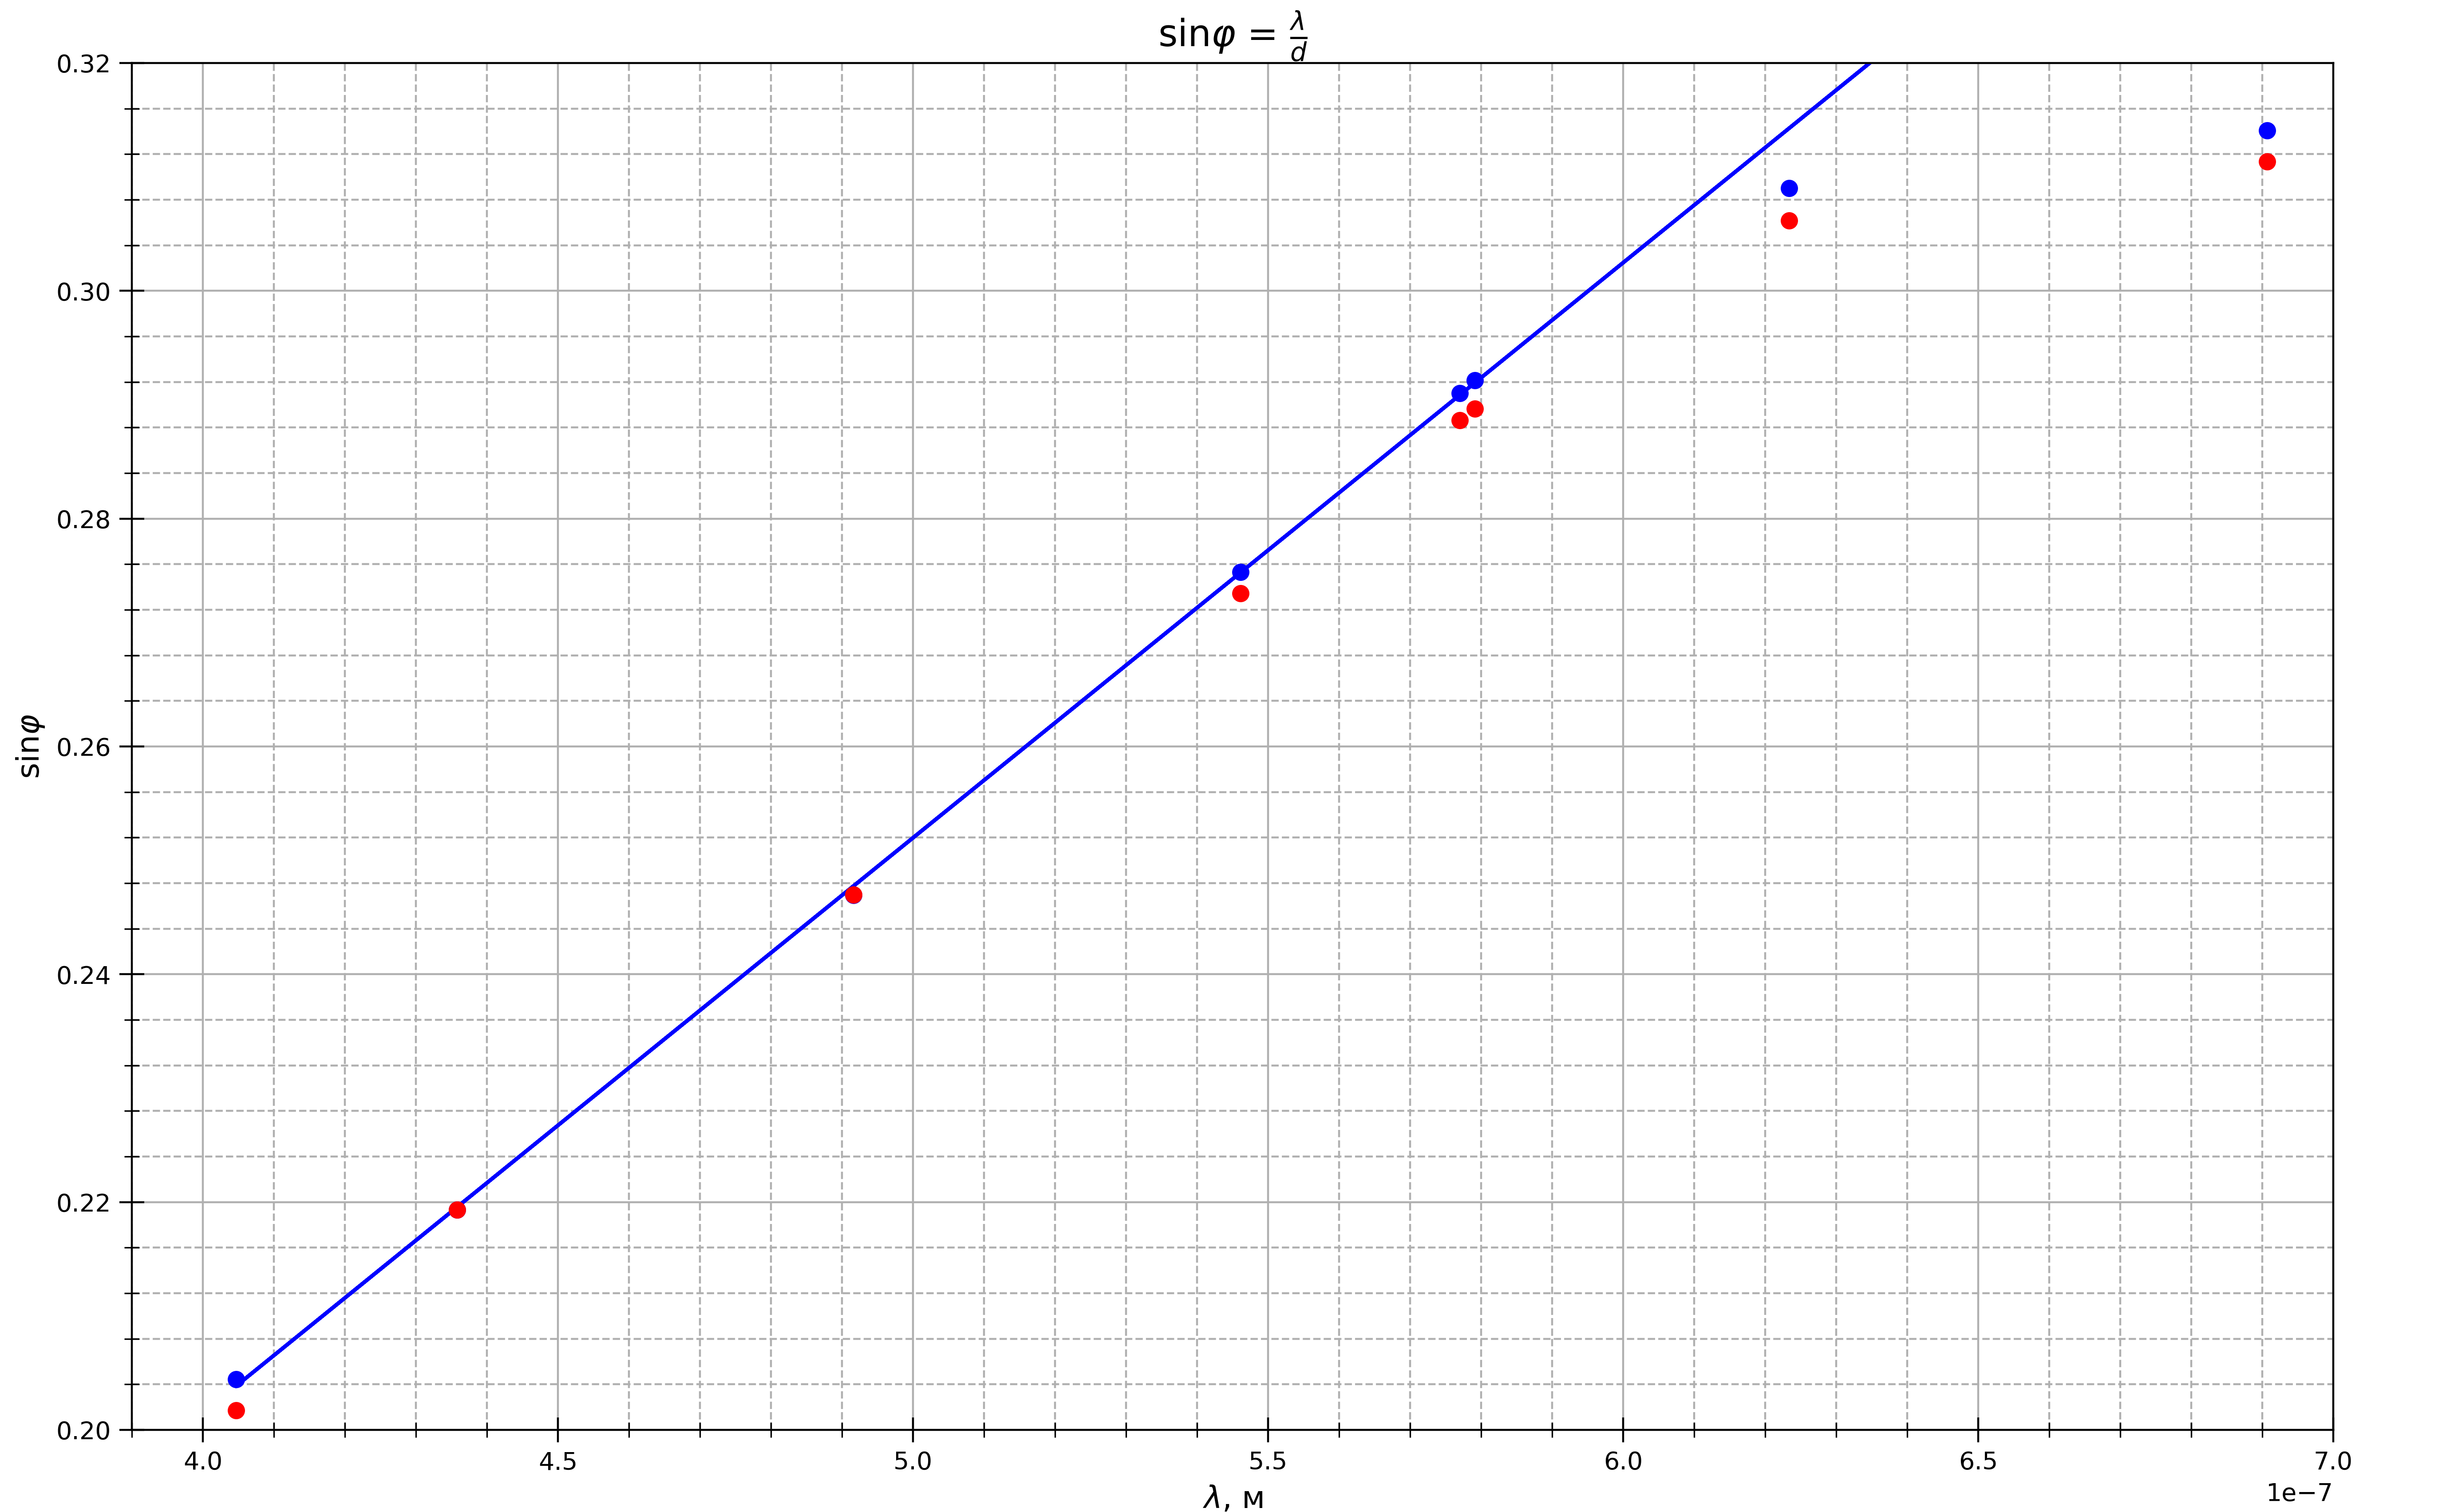
\includegraphics[width=0.85\linewidth]{graph1'.png}
\caption{график зависимости $\text{sin} \varphi_{m}=\frac{\lambda}{d}$}
\label{fig:mpr}
\end{figure}
\newpage
\subparagraph{2.} Рассчитаем экспериментальную угловую дисперсию для жёлтой пары $D=\frac{d\varphi}{d\lambda}$ в спектрах разного порядка и сравним с рассчитанной по формуле: $D=\frac{m}{d\text{cos}\varphi_{m}}$. Результаты приведены в таблице 1.


\begin{table}[H]
\begin{center}
			\caption{}
			\label{Таблица 2}
			\begin{tabular}{|r|c|c|c|}
				\hline
				$m$  & $ \Delta \varphi , ''$  & $D_{эксп}$,  $ 10^{-5} $ рад/$  \buildrel _{\circ} \over {\mathrm{A}}$   & $D_{теор}$,   $ 10^{-5} $ рад/$  \buildrel _{\circ} \over {\mathrm{A}}$   \\ \hline
				1  &215    & $4,96\pm 0,02$ & $5,05$  \\ \hline
				-1 & 237     &$-5,47\pm 0,02$ & $-5,05$ \\ \hline
				2  & 525    &$12,12\pm0,02$ & $12.5$  \\ \hline
				-2 & 570     &$-13,16\pm 0,02$ & $-12.5$ \\ \hline
			\end{tabular}
   \end{center}
		\end{table}

\subparagraph{3.} Найдём разрешающую способность $R=\frac{\varphi}{\delta \varphi}=\frac{\lambda}{\delta \lambda}$, где $\delta \lambda$ можно найти из $\Delta \varphi \approx D \delta \lambda$

\begin{center}
    $\delta \lambda \approx 2,1 ~ мкм$
\end{center}

\begin{center}
    $R= 289$
\end{center}

Число эффективно работающих штрихов и размер освещённой части решётки:

\begin{center}
    $N=\frac{R}{m}=289$
\end{center}

\begin{center}
    $l = d\cdot N=0,6~мм$
\end{center}
\paragraph{Вывод:} в данной лабораторной работе мы отъюстировали гониометр, исследовали спектр ртутной лампы и дисперсию амплитудной решётки. Нашли шаг решётки $d = 1,98\pm 0,02 ~ мкм$. Угловая дисперсия, которую мы вычислили экспериментально, близка к теоретической. Также мы вычислили разрешающую способность и эффективную часть решётки.
\end{document}
